\subsection*{Problema 36}

\textbf{Enunciado:}
Calcular la integral indefinida:
\begin{align*}
\int \dfrac{2x^4 + 3x^3 - x - 1}{(x - 1)(x^2 + 2x + 2)^2} \, dx
\end{align*}

\textbf{Solución:}
El integrando es una función racional propia. 
Utilizamos el método de fracciones parciales 
con la descomposición indicada:

\begin{align*}
\dfrac{2x^4 + 3x^3 - x - 1}{(x - 1)(x^2 + 2x + 2)^2} &= 
\dfrac{A}{x - 1} \\
&+ \dfrac{Bx + C}{x^2 + 2x + 2} \\
&+ \dfrac{Dx + E}{(x^2 + 2x + 2)^2}
\end{align*}

Multiplicando ambos lados por el denominador 
común, obtenemos la identidad polinómica. 
Evaluando en $x = 1$, determinamos el coeficiente:
\begin{align*}
A &= \dfrac{2(1)^4 + 3(1)^3 - 1 - 1}{(1^2 + 2(1) + 2)^2} \\
&= \dfrac{3}{5^2} = \dfrac{3}{25}
\end{align*}

Expandiendo y agrupando términos semejantes para 
los coeficientes restantes, hallamos:
\begin{align*}
B &= \dfrac{47}{25}, \quad C = -\dfrac{4}{25} \\
D &= \dfrac{3}{5}, \quad E = -\dfrac{1}{5}
\end{align*}

Sustituyendo los valores, la integral se 
descompone en tres partes:
\begin{align*}
\int \dfrac{3/25}{x - 1} \, dx 
&+ \int \dfrac{\frac{47}{25}x - \frac{4}{25}}{x^2 + 2x + 2} \, dx \\
&+ \int \dfrac{\frac{3}{5}x - \frac{1}{5}}{(x^2 + 2x + 2)^2} \, dx
\end{align*}

La primera integral es inmediata:
\begin{align*}
\int \dfrac{3/25}{x - 1} \, dx = \dfrac{3}{25} \ln|x - 1|
\end{align*}

Para la segunda integral, reescribimos el 
numerador usando la derivada del denominador 
$2x + 2$:
\begin{align*}
\dfrac{47}{50} \int \dfrac{2x + 2}{x^2 + 2x + 2} \, dx 
- \dfrac{107}{50} \int \dfrac{1}{(x + 1)^2 + 1} \, dx
\end{align*}
Esto resulta en:
\begin{align*}
\dfrac{47}{50} \ln(x^2 + 2x + 2) - \dfrac{107}{50} \arctan(x + 1)
\end{align*}

Para la tercera integral, aplicamos la 
sustitución trigonométrica $x + 1 = \tan(\theta)$, 
con lo cual $dx = \sec^2(\theta) \, d\theta$:
\begin{align*}
\int \dfrac{\frac{3}{5}(\tan\theta - 1)}{\sec^4(\theta)} \sec^2(\theta) \, d\theta 
&= \dfrac{3}{5} \int \dfrac{\sin\theta - \cos\theta}{\sec^2(\theta)} \, d\theta \\
&= -\dfrac{3}{10}\cos^2\theta - \dfrac{3}{10}(\theta + \sin\theta\cos\theta)
\end{align*}

Retornando a la variable original $x$ y 
sumando todas las antiderivadas, obtenemos 
la solución general con $C$ como constante de integración:
\begin{align*}
F(x) &= \dfrac{3}{25}\ln|x - 1| 
+ \dfrac{47}{50}\ln(x^2 + 2x + 2) \\
&- \dfrac{107}{50}\arctan(x + 1) \\
&- \dfrac{3}{5(x^2 + 2x + 2)} + C
\end{align*}

\begin{figure}[H]
	\centering
	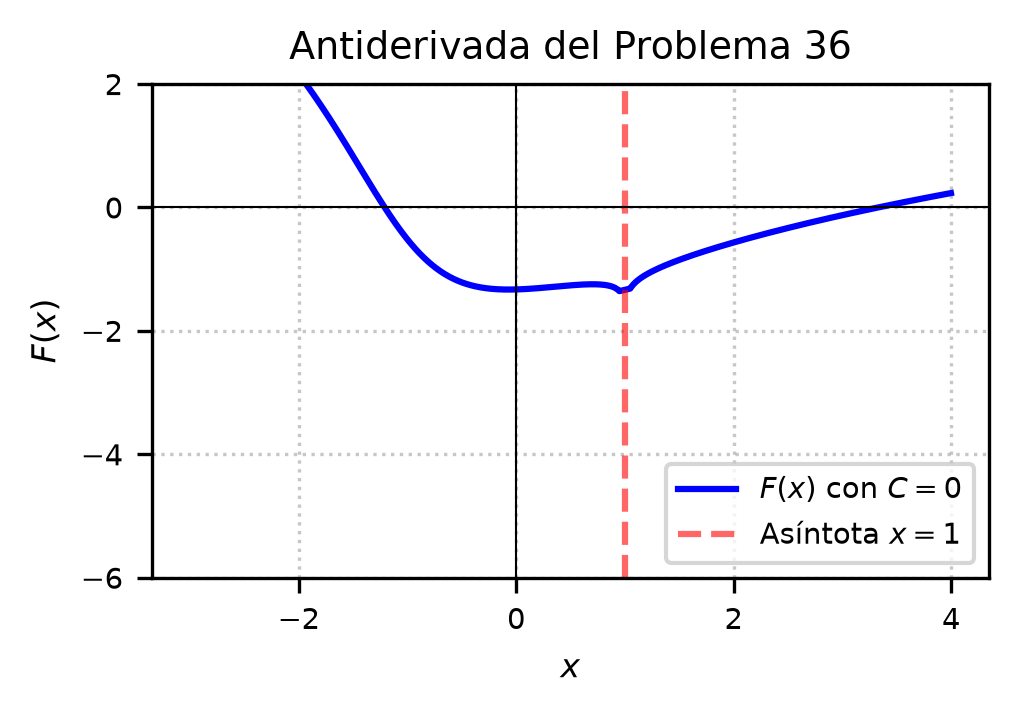
\includegraphics[width=\columnwidth]{semana_03/graficas/SEM03_P36_grafica.png}
	\caption{Representación gráfica de $f(x)$ y su antiderivada $F(x)$ evaluada para la constante de integración $C = 0$ (Problema 36).}
	\label{fig:problema36}
\end{figure}
